\documentclass{standalone}
\usepackage{tikz}
\usetikzlibrary{patterns, positioning}

\begin{document}
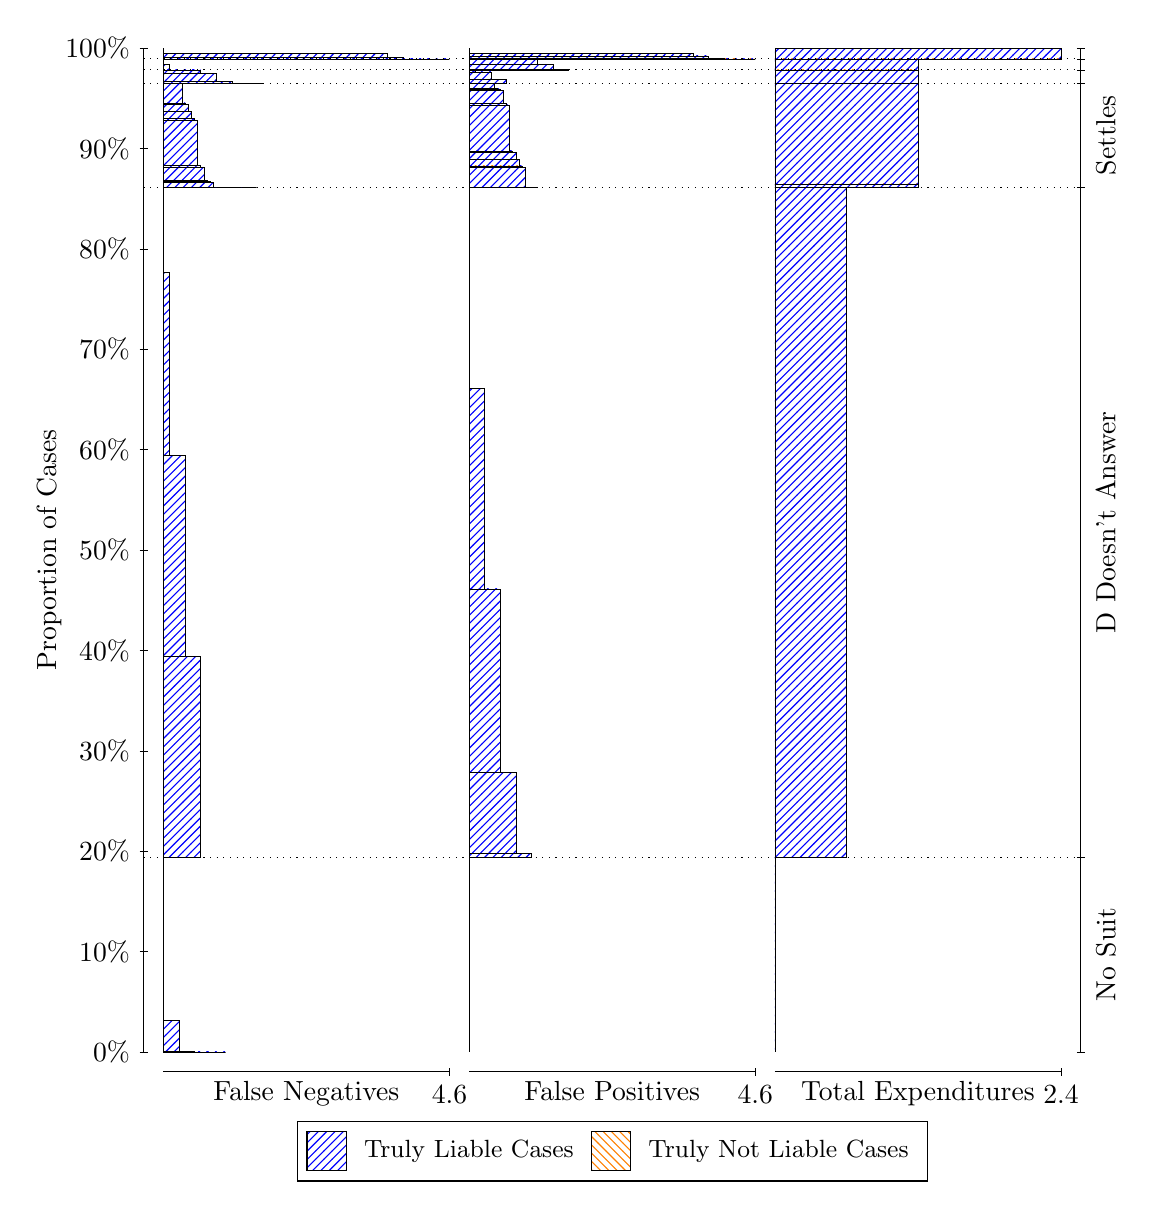
\begin{tikzpicture}
\draw[black, very thin] (1.5,1.75) -- (1.5,14.5);
\node[rotate=90, anchor=center] at (0.3, 8.125) {Proportion of Cases};
\draw[black, very thin] (1.45,1.75) -- (1.55,1.75);
\node[anchor=east] at (1.45, 1.75) {0\%};
\draw[black, very thin] (1.45,3.025) -- (1.55,3.025);
\node[anchor=east] at (1.45, 3.025) {10\%};
\draw[black, very thin] (1.45,4.3) -- (1.55,4.3);
\node[anchor=east] at (1.45, 4.3) {20\%};
\draw[black, very thin] (1.45,5.575) -- (1.55,5.575);
\node[anchor=east] at (1.45, 5.575) {30\%};
\draw[black, very thin] (1.45,6.85) -- (1.55,6.85);
\node[anchor=east] at (1.45, 6.85) {40\%};
\draw[black, very thin] (1.45,8.125) -- (1.55,8.125);
\node[anchor=east] at (1.45, 8.125) {50\%};
\draw[black, very thin] (1.45,9.4) -- (1.55,9.4);
\node[anchor=east] at (1.45, 9.4) {60\%};
\draw[black, very thin] (1.45,10.675) -- (1.55,10.675);
\node[anchor=east] at (1.45, 10.675) {70\%};
\draw[black, very thin] (1.45,11.95) -- (1.55,11.95);
\node[anchor=east] at (1.45, 11.95) {80\%};
\draw[black, very thin] (1.45,13.225) -- (1.55,13.225);
\node[anchor=east] at (1.45, 13.225) {90\%};
\draw[black, very thin] (1.45,14.5) -- (1.55,14.5);
\node[anchor=east] at (1.45, 14.5) {100\%};

\draw[black, very thin] (13.4,1.75) -- (13.4,14.5);
\draw[black, very thin] (13.35,1.75) -- (13.45,1.75);
\node[anchor=west] at (13.35, 1.75) {};
\draw[black, very thin] (13.35,4.2243) -- (13.45,4.2243);
\node[anchor=west] at (13.35, 4.2243) {};
\draw[black, very thin] (13.35,12.728) -- (13.45,12.728);
\node[anchor=west] at (13.35, 12.728) {};
\draw[black, very thin] (13.35,14.055) -- (13.45,14.055);
\node[anchor=west] at (13.35, 14.055) {};
\draw[black, very thin] (13.35,14.222) -- (13.45,14.222);
\node[anchor=west] at (13.35, 14.222) {};
\draw[black, very thin] (13.35,14.362) -- (13.45,14.362);
\node[anchor=west] at (13.35, 14.362) {};
\draw[black, very thin] (13.35,14.5) -- (13.45,14.5);
\node[anchor=west] at (13.35, 14.5) {};

\draw[black, very thin, pattern color=blue, pattern=north east lines] (1.75,1.75) rectangle (2.5399,1.75);
\draw[black, very thin, pattern color=blue, pattern=north east lines] (1.75,1.75) rectangle (2.3424,1.75);
\draw[black, very thin, pattern color=blue, pattern=north east lines] (1.75,1.75) rectangle (2.1449,1.7535);
\draw[black, very thin, pattern color=blue, pattern=north east lines] (1.75,1.7535) rectangle (1.9475,2.1551);
\draw[black, very thin, pattern color=orange, pattern=north west lines] (1.75,2.1551) rectangle (1.75,2.1551);
\draw[black, very thin, pattern color=blue, pattern=north east lines] (1.75,2.1551) rectangle (1.75,4.2243);
\draw[black, very thin, pattern color=blue, pattern=north east lines] (1.75,4.2243) rectangle (2.2239,6.7742);
\draw[black, very thin, pattern color=blue, pattern=north east lines] (1.75,6.7742) rectangle (2.0264,9.3224);
\draw[black, very thin, pattern color=blue, pattern=north east lines] (1.75,9.3224) rectangle (1.829,11.653);
\draw[black, very thin, pattern color=orange, pattern=north west lines] (1.75,11.653) rectangle (1.75,11.653);
\draw[black, very thin, pattern color=blue, pattern=north east lines] (1.75,11.653) rectangle (1.75,12.728);
\draw[black, very thin, pattern color=blue, pattern=north east lines] (1.75,12.728) rectangle (2.9348,12.728);
\draw[black, very thin, pattern color=blue, pattern=north east lines] (1.75,12.728) rectangle (2.8558,12.728);
\draw[black, very thin, pattern color=blue, pattern=north east lines] (1.75,12.728) rectangle (2.7768,12.728);
\draw[black, very thin, pattern color=blue, pattern=north east lines] (1.75,12.728) rectangle (2.7373,12.728);
\draw[black, very thin, pattern color=blue, pattern=north east lines] (1.75,12.728) rectangle (2.6978,12.728);
\draw[black, very thin, pattern color=blue, pattern=north east lines] (1.75,12.728) rectangle (2.6583,12.728);
\draw[black, very thin, pattern color=blue, pattern=north east lines] (1.75,12.728) rectangle (2.6188,12.728);
\draw[black, very thin, pattern color=blue, pattern=north east lines] (1.75,12.728) rectangle (2.5793,12.728);
\draw[black, very thin, pattern color=blue, pattern=north east lines] (1.75,12.728) rectangle (2.5399,12.729);
\draw[black, very thin, pattern color=blue, pattern=north east lines] (1.75,12.729) rectangle (2.5004,12.729);
\draw[black, very thin, pattern color=blue, pattern=north east lines] (1.75,12.729) rectangle (2.4609,12.735);
\draw[black, very thin, pattern color=blue, pattern=north east lines] (1.75,12.735) rectangle (2.4214,12.735);
\draw[black, very thin, pattern color=blue, pattern=north east lines] (1.75,12.735) rectangle (2.3819,12.792);
\draw[black, very thin, pattern color=blue, pattern=north east lines] (1.75,12.792) rectangle (2.3424,12.804);
\draw[black, very thin, pattern color=blue, pattern=north east lines] (1.75,12.804) rectangle (2.3029,12.818);
\draw[black, very thin, pattern color=blue, pattern=north east lines] (1.75,12.818) rectangle (2.2634,12.982);
\draw[black, very thin, pattern color=blue, pattern=north east lines] (1.75,12.982) rectangle (2.2239,13.006);
\draw[black, very thin, pattern color=blue, pattern=north east lines] (1.75,13.006) rectangle (2.1844,13.588);
\draw[black, very thin, pattern color=blue, pattern=north east lines] (1.75,13.588) rectangle (2.1449,13.604);
\draw[black, very thin, pattern color=blue, pattern=north east lines] (1.75,13.604) rectangle (2.1054,13.7);
\draw[black, very thin, pattern color=blue, pattern=north east lines] (1.75,13.7) rectangle (2.0659,13.78);
\draw[black, very thin, pattern color=blue, pattern=north east lines] (1.75,13.78) rectangle (2.0264,13.803);
\draw[black, very thin, pattern color=blue, pattern=north east lines] (1.75,13.803) rectangle (1.987,14.048);
\draw[black, very thin, pattern color=blue, pattern=north east lines] (1.75,14.048) rectangle (1.908,14.055);
\draw[black, very thin, pattern color=blue, pattern=north east lines] (1.75,14.055) rectangle (1.829,14.055);
\draw[black, very thin, pattern color=orange, pattern=north west lines] (1.75,14.055) rectangle (1.75,14.055);
\draw[black, very thin, pattern color=blue, pattern=north east lines] (1.75,14.055) rectangle (3.0138,14.055);
\draw[black, very thin, pattern color=blue, pattern=north east lines] (1.75,14.055) rectangle (2.8163,14.055);
\draw[black, very thin, pattern color=blue, pattern=north east lines] (1.75,14.055) rectangle (2.6188,14.08);
\draw[black, very thin, pattern color=blue, pattern=north east lines] (1.75,14.08) rectangle (2.4214,14.18);
\draw[black, very thin, pattern color=blue, pattern=north east lines] (1.75,14.18) rectangle (2.2239,14.222);
\draw[black, very thin, pattern color=orange, pattern=north west lines] (1.75,14.222) rectangle (1.75,14.222);
\draw[black, very thin, pattern color=blue, pattern=north east lines] (1.75,14.222) rectangle (2.2239,14.222);
\draw[black, very thin, pattern color=blue, pattern=north east lines] (1.75,14.222) rectangle (2.0264,14.223);
\draw[black, very thin, pattern color=blue, pattern=north east lines] (1.75,14.223) rectangle (1.829,14.293);
\draw[black, very thin, pattern color=orange, pattern=north west lines] (1.75,14.293) rectangle (1.75,14.293);
\draw[black, very thin, pattern color=blue, pattern=north east lines] (1.75,14.293) rectangle (1.75,14.362);
\draw[black, very thin, pattern color=blue, pattern=north east lines] (1.75,14.362) rectangle (5.3833,14.362);
\draw[black, very thin, pattern color=blue, pattern=north east lines] (1.75,14.362) rectangle (5.1859,14.362);
\draw[black, very thin, pattern color=blue, pattern=north east lines] (1.75,14.362) rectangle (4.9884,14.362);
\draw[black, very thin, pattern color=blue, pattern=north east lines] (1.75,14.362) rectangle (4.7909,14.384);
\draw[black, very thin, pattern color=blue, pattern=north east lines] (1.75,14.384) rectangle (4.5935,14.431);
\draw[black, very thin, pattern color=blue, pattern=north east lines] (1.75,14.431) rectangle (4.396,14.431);
\draw[black, very thin, pattern color=blue, pattern=north east lines] (1.75,14.431) rectangle (4.1986,14.431);
\draw[black, very thin, pattern color=orange, pattern=north west lines] (1.75,14.431) rectangle (1.75,14.431);
\draw[black, very thin, pattern color=blue, pattern=north east lines] (1.75,14.431) rectangle (1.75,14.5);
\draw[black, very thin, pattern color=orange, pattern=north west lines] (5.6333,1.75) rectangle (5.6333,1.75);
\draw[black, very thin, pattern color=blue, pattern=north east lines] (5.6333,1.75) rectangle (5.6333,4.2243);
\draw[black, very thin, pattern color=orange, pattern=north west lines] (5.6333,4.2243) rectangle (6.4232,4.2243);
\draw[black, very thin, pattern color=blue, pattern=north east lines] (5.6333,4.2243) rectangle (6.4232,4.2673);
\draw[black, very thin, pattern color=blue, pattern=north east lines] (5.6333,4.2673) rectangle (6.2257,5.2993);
\draw[black, very thin, pattern color=blue, pattern=north east lines] (5.6333,5.2993) rectangle (6.0283,7.6303);
\draw[black, very thin, pattern color=blue, pattern=north east lines] (5.6333,7.6303) rectangle (5.8308,10.178);
\draw[black, very thin, pattern color=blue, pattern=north east lines] (5.6333,10.178) rectangle (5.6333,12.728);
\draw[black, very thin, pattern color=orange, pattern=north west lines] (5.6333,12.728) rectangle (6.5022,12.728);
\draw[black, very thin, pattern color=blue, pattern=north east lines] (5.6333,12.728) rectangle (6.5022,12.729);
\draw[black, very thin, pattern color=orange, pattern=north west lines] (5.6333,12.729) rectangle (6.4232,12.729);
\draw[black, very thin, pattern color=blue, pattern=north east lines] (5.6333,12.729) rectangle (6.4232,12.735);
\draw[black, very thin, pattern color=orange, pattern=north west lines] (5.6333,12.735) rectangle (6.3442,12.735);
\draw[black, very thin, pattern color=blue, pattern=north east lines] (5.6333,12.735) rectangle (6.3442,12.981);
\draw[black, very thin, pattern color=blue, pattern=north east lines] (5.6333,12.981) rectangle (6.3047,13.004);
\draw[black, very thin, pattern color=orange, pattern=north west lines] (5.6333,13.004) rectangle (6.2652,13.004);
\draw[black, very thin, pattern color=blue, pattern=north east lines] (5.6333,13.004) rectangle (6.2652,13.084);
\draw[black, very thin, pattern color=blue, pattern=north east lines] (5.6333,13.084) rectangle (6.2257,13.179);
\draw[black, very thin, pattern color=orange, pattern=north west lines] (5.6333,13.179) rectangle (6.1862,13.179);
\draw[black, very thin, pattern color=blue, pattern=north east lines] (5.6333,13.179) rectangle (6.1862,13.195);
\draw[black, very thin, pattern color=blue, pattern=north east lines] (5.6333,13.195) rectangle (6.1467,13.778);
\draw[black, very thin, pattern color=blue, pattern=north east lines] (5.6333,13.778) rectangle (6.1072,13.801);
\draw[black, very thin, pattern color=blue, pattern=north east lines] (5.6333,13.801) rectangle (6.0678,13.966);
\draw[black, very thin, pattern color=blue, pattern=north east lines] (5.6333,13.966) rectangle (6.0283,13.98);
\draw[black, very thin, pattern color=blue, pattern=north east lines] (5.6333,13.98) rectangle (5.9888,13.991);
\draw[black, very thin, pattern color=blue, pattern=north east lines] (5.6333,13.991) rectangle (5.9493,14.049);
\draw[black, very thin, pattern color=blue, pattern=north east lines] (5.6333,14.049) rectangle (5.9098,14.049);
\draw[black, very thin, pattern color=blue, pattern=north east lines] (5.6333,14.049) rectangle (5.8703,14.055);
\draw[black, very thin, pattern color=blue, pattern=north east lines] (5.6333,14.055) rectangle (5.8308,14.055);
\draw[black, very thin, pattern color=blue, pattern=north east lines] (5.6333,14.055) rectangle (5.7913,14.055);
\draw[black, very thin, pattern color=blue, pattern=north east lines] (5.6333,14.055) rectangle (5.7518,14.055);
\draw[black, very thin, pattern color=blue, pattern=north east lines] (5.6333,14.055) rectangle (5.7123,14.055);
\draw[black, very thin, pattern color=blue, pattern=north east lines] (5.6333,14.055) rectangle (5.6728,14.055);
\draw[black, very thin, pattern color=blue, pattern=north east lines] (5.6333,14.055) rectangle (5.6333,14.055);
\draw[black, very thin, pattern color=orange, pattern=north west lines] (5.6333,14.055) rectangle (6.1072,14.055);
\draw[black, very thin, pattern color=blue, pattern=north east lines] (5.6333,14.055) rectangle (6.1072,14.097);
\draw[black, very thin, pattern color=blue, pattern=north east lines] (5.6333,14.097) rectangle (5.9098,14.197);
\draw[black, very thin, pattern color=blue, pattern=north east lines] (5.6333,14.197) rectangle (5.7123,14.222);
\draw[black, very thin, pattern color=blue, pattern=north east lines] (5.6333,14.222) rectangle (5.6333,14.222);
\draw[black, very thin, pattern color=orange, pattern=north west lines] (5.6333,14.222) rectangle (6.8971,14.222);
\draw[black, very thin, pattern color=blue, pattern=north east lines] (5.6333,14.222) rectangle (6.8971,14.224);
\draw[black, very thin, pattern color=blue, pattern=north east lines] (5.6333,14.224) rectangle (6.6996,14.291);
\draw[black, very thin, pattern color=blue, pattern=north east lines] (5.6333,14.291) rectangle (6.5022,14.361);
\draw[black, very thin, pattern color=blue, pattern=north east lines] (5.6333,14.361) rectangle (6.3047,14.362);
\draw[black, very thin, pattern color=blue, pattern=north east lines] (5.6333,14.362) rectangle (6.1072,14.362);
\draw[black, very thin, pattern color=orange, pattern=north west lines] (5.6333,14.362) rectangle (9.2667,14.362);
\draw[black, very thin, pattern color=blue, pattern=north east lines] (5.6333,14.362) rectangle (9.2667,14.362);
\draw[black, very thin, pattern color=orange, pattern=north west lines] (5.6333,14.362) rectangle (9.0692,14.362);
\draw[black, very thin, pattern color=blue, pattern=north east lines] (5.6333,14.362) rectangle (9.0692,14.362);
\draw[black, very thin, pattern color=orange, pattern=north west lines] (5.6333,14.362) rectangle (8.8717,14.362);
\draw[black, very thin, pattern color=blue, pattern=north east lines] (5.6333,14.362) rectangle (8.8717,14.365);
\draw[black, very thin, pattern color=orange, pattern=north west lines] (5.6333,14.365) rectangle (8.6743,14.365);
\draw[black, very thin, pattern color=blue, pattern=north east lines] (5.6333,14.365) rectangle (8.6743,14.401);
\draw[black, very thin, pattern color=blue, pattern=north east lines] (5.6333,14.401) rectangle (8.4768,14.43);
\draw[black, very thin, pattern color=blue, pattern=north east lines] (5.6333,14.43) rectangle (8.2793,14.431);
\draw[black, very thin, pattern color=blue, pattern=north east lines] (5.6333,14.431) rectangle (8.0819,14.431);
\draw[black, very thin, pattern color=blue, pattern=north east lines] (5.6333,14.431) rectangle (7.8844,14.431);
\draw[black, very thin, pattern color=orange, pattern=north west lines] (5.6333,14.431) rectangle (5.6333,14.431);
\draw[black, very thin, pattern color=blue, pattern=north east lines] (5.6333,14.431) rectangle (5.6333,14.5);
\draw[black, very thin, pattern color=orange, pattern=north west lines] (9.5167,1.75) rectangle (9.5167,1.75);
\draw[black, very thin, pattern color=blue, pattern=north east lines] (9.5167,1.75) rectangle (9.5167,4.2243);
\draw[black, very thin, pattern color=orange, pattern=north west lines] (9.5167,4.2243) rectangle (10.425,4.2243);
\draw[black, very thin, pattern color=blue, pattern=north east lines] (9.5167,4.2243) rectangle (10.425,12.728);
\draw[black, very thin, pattern color=orange, pattern=north west lines] (9.5167,12.728) rectangle (11.333,12.728);
\draw[black, very thin, pattern color=blue, pattern=north east lines] (9.5167,12.728) rectangle (11.333,12.775);
\draw[black, very thin, pattern color=orange, pattern=north west lines] (9.5167,12.775) rectangle (11.333,12.775);
\draw[black, very thin, pattern color=blue, pattern=north east lines] (9.5167,12.775) rectangle (11.333,14.055);
\draw[black, very thin, pattern color=orange, pattern=north west lines] (9.5167,14.055) rectangle (11.333,14.055);
\draw[black, very thin, pattern color=blue, pattern=north east lines] (9.5167,14.055) rectangle (11.333,14.222);
\draw[black, very thin, pattern color=orange, pattern=north west lines] (9.5167,14.222) rectangle (11.333,14.222);
\draw[black, very thin, pattern color=blue, pattern=north east lines] (9.5167,14.222) rectangle (11.333,14.362);
\draw[black, very thin, pattern color=orange, pattern=north west lines] (9.5167,14.362) rectangle (13.15,14.362);
\draw[black, very thin, pattern color=blue, pattern=north east lines] (9.5167,14.362) rectangle (13.15,14.5);
\draw[black, dotted] (1.5,4.2243) -- (13.4,4.2243);
\draw[black, dotted] (1.5,12.728) -- (13.4,12.728);
\draw[black, dotted] (1.5,14.055) -- (13.4,14.055);
\draw[black, dotted] (1.5,14.222) -- (13.4,14.222);
\draw[black, dotted] (1.5,14.362) -- (13.4,14.362);
\draw[black, very thin] (1.75,1.5) -- (5.3833,1.5);
\node[anchor=north] at (3.5667, 1.5) {False Negatives};
\draw[black, very thin] (5.3833,1.45) -- (5.3833,1.55);
\node[anchor=north] at (5.3833, 1.45) {4.6};

\draw[black, very thin] (5.6333,1.5) -- (9.2667,1.5);
\node[anchor=north] at (7.45, 1.5) {False Positives};
\draw[black, very thin] (9.2667,1.45) -- (9.2667,1.55);
\node[anchor=north] at (9.2667, 1.45) {4.6};

\draw[black, very thin] (9.5167,1.5) -- (13.15,1.5);
\node[anchor=north] at (11.333, 1.5) {Total Expenditures};
\draw[black, very thin] (13.15,1.45) -- (13.15,1.55);
\node[anchor=north] at (13.15, 1.45) {2.4};

\node[black, centered, rotate=90] at (13.72, 2.9871) {No Suit};
\node[black, centered, rotate=90] at (13.72, 8.4763) {D Doesn't Answer};
\node[black, centered, rotate=90] at (13.72, 13.392) {Settles};




\draw (7.449999999999999,1.5) node[draw=none] (baseCoordinate) {};
\begin{scope}[align=center]
        \matrix[scale=0.5, draw=black, below=0.5cm of baseCoordinate, nodes={draw}, column sep=0.1cm]{
            \node[rectangle, draw, minimum width=0.5cm, minimum height=0.5cm, pattern=north east lines, pattern color=blue] {}; &
            \node[draw=none, font=\small] (B) {Truly Liable Cases}; &
            \node[rectangle, draw, minimum width=0.5cm, minimum height=0.5cm, pattern=north west lines, pattern color=orange] {}; &
            \node[draw=none, font=\small] (B) {Truly Not Liable Cases}; \\
            };
\end{scope}

\end{tikzpicture}
\end{document}